\documentclass{ximera}
\graphicspath{
{./}
{volumes/}
{arclengths/}
{centroids/}
{techniques/}
{applications/}
{series/}
{powerseries/}
{odes/}
{lessons/}
}
\usepackage{booktabs}

\newcommand{\bigmath}[1]{$\displaystyle #1$}
\newcommand{\choicebreak}{}
\newenvironment{type}{}{}
\newenvironment{notes}{}{}
\newenvironment{keywords}{}{}
\newcommand{\offline}{}
\newenvironment{comments}{\begin{feedback}}{\end{feedback}}
\newenvironment{multiplechoice}{\begin{multipleChoice}}{\end{multipleChoice}}
\title{Probability}
%%%%%\author{Philip T. Gressman}

\begin{document}
\begin{abstract}
  A brief introduction to the calculus of continuous random variables.
\end{abstract}
\maketitle


A \textbf{random variable} is a quantity whose value depends on the outcome of some random event or process:
\begin{itemize}
\item When rolling a six-sided die, there is a random variable $X$ associated to this action which represents the side of the die that comes up on top. In this case, possible values of $X$ are $1,2,3,4,5,$ or $6$, and (if it's a fair die) each outcome is equally likely. This is an example of a \textbf{discrete} random variable, which means that the possible values are finite or otherwise clearly separated from one another.
\item For any given brand of lightbulb, there is an associated random variable $T$ which represents the lifetime of the bulb (i.e., $T$ equals the total time that a particular bulb lasts before it burns out). We idealize this random variable to be a \textbf{continuous} random variable, because the lifetime could be any positive amount of time in principle (i.e., we might have one bulb lasting $1000.0423$ hours and another lasting only $10^{-9}$ seconds longer than that).
\end{itemize}

We will focus primarily on continuous random variables. The information we will typically need to know in order to work with continuous random variables are:
\begin{itemize}
\item The interval $I$ of possible values that the random variable may take. For the lightbulb burn-out example, this would be the interval $[0,\infty)$.
\item A \textbf{probability density function} to compute the probability of various events.
\end{itemize}
\begin{definition}
A probability density function $f$ on an interval $[a,b]$ is a function which is
\begin{enumerate}
\item Non-negative, i.e., $f(x) \geq 0$ for every $x$ in the interval $[a,b]$,
\item Can be integrated on the interval $[a,b]$; this is possible if, for example, $f$ is continuous on $[a,b]$,
\item Has total integral $1$, i.e.,
\[ \int_a^b f(x) dx = 1. \]
(Note: we can allow $a = -\infty$ and/or $b = \infty$ if these make sense for a particular random variable. In this case, we interpret the integral as an improper integral.)
\end{enumerate}
\end{definition}
As the name suggests, a PDF $f(x)$ represents a density of probability; so if $f(x)$ is relatively large at a particular value of $x$, this indicates that values near that $x$ are relatively more likely to occur than values near where $f(x)$ is smaller.

\begin{definition}
Suppose $X$ is a random variable taking values between $a$ and $b$ which has a probability density function $f(x)$ on the interval $[a,b]$.
 Then for any two numbers $c \leq d$ inside the interval $[a,b]$, the probability that $X$ takes a value between $c$ and $d$ is given by integration:
 \[ P( c \leq X \leq d) = \int_c^d f(x) dx. \]
 \begin{center}
 \begin{image}
 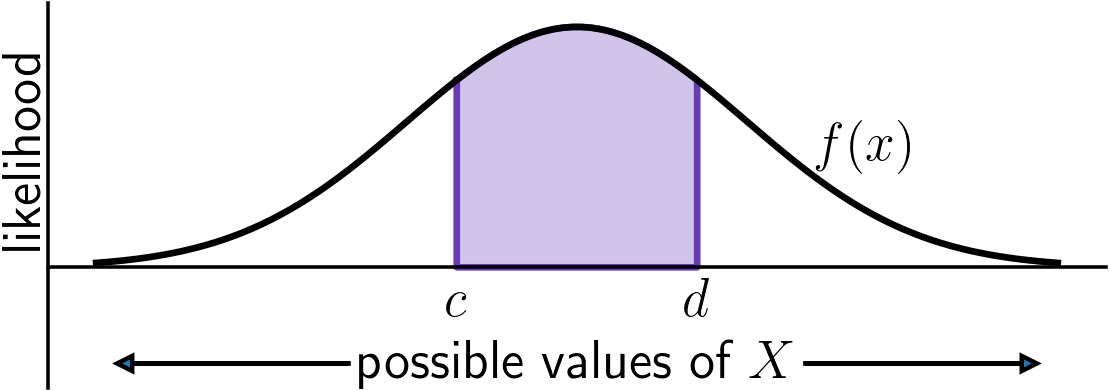
\includegraphics[width=4in]{probability01.png}
 \end{image}
 {\footnotesize When plotting a PDF, the horizontal axis ranges over possible values of the random variable $X$ and the vertical axis measures relatively likelihood. The area under the graph equals the probability that $X$ takes values between $c$ and $d$.}
 \end{center}
 \end{definition}



\end{document}
